\section{Теоритические сведения}
\begin{figure}[ht!]
    \center{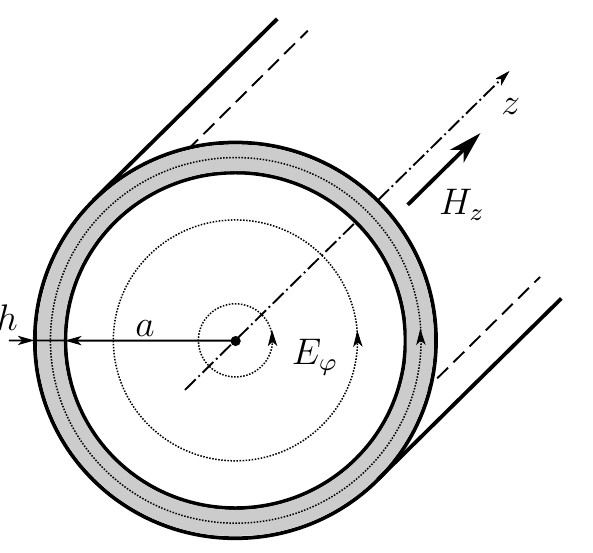
\includegraphics[width=0.8\linewidth]{../img/fig1.png}}
\end{figure}
В работе изучается скин-эффект в длинном тонкостенном медном цилиндре, помещённом внутрь соленоида.

Пусть цилиндр достаточно длинный, так что в нём можно пренебречь краевыми эффектами. В
этом приближении магнитное поле $\vec{H}$ всюду направлено по оси системы,
а вихревое электрическое поле $\vec{E}$  будет всюду перпендикулярно радиусу.
Все величины будем считать колеблющимися по гармоническому закону с некоторой частотой
$w$. Тогда
\[
    H_{z} = H(r)e^{iwt}
\]
\[
    E_{ \varphi} = E(r)e^{iwt}
\]
где $H(r)$ и $E(r)$~--- комплексные амплитуды колебаний соответствующих полей, зависящие только от
расстояния $r$ до оси системы. Заметим, что на границе цилиндра должны быть непрерывны касательные
к поверхности компоненты как $\vec{E}$, так и $\vec{B}$, поэтому $E(r)$ и $H(r)$ непрерывны во всей исследуемой области.

Пусть длинный полый цилиндр имеет радиус $a$ и толщину стенки $h \ll a$.
Последнее условие позволяет для описания поля внутри стенки ограничиться одномерным приближением.
При этом для полного решения задачи необходимо вычислить и распределение
поля внутри цилиндра.

Поскольку внутри цилиндра ток отсутствует, магнитное поле там является однородным
\[
    H_{z}(r, t) = H_{1}e^{iwt}
\]
где $H_{1}=\text{const}$~--- амплитуда поля на внутренней поверхности цилиндра. Для нахождения вихревого электрического
поля воспользуемся законом электромагнитной индукции  в интегральной форме:
\[
    E(r) = -\frac{1}{2}\mu_{0}r\cdot iwH_{1}
\]
Отсюда получим связь амплитуд колебаний электрического и магнитного полей на внутренней
 границе цилиндра:
 \[
     E_{1} = -\frac{1}{2}iwa\mu_{0}H_{1} 
 \]
\begin{figure}[ht!]
    \center{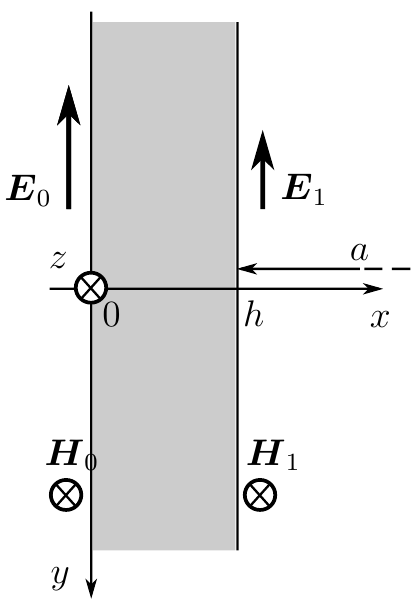
\includegraphics[width=0.5\linewidth]{../img/fig2.png}}
\end{figure}

Поле внутри тонкой стенки цилиндра описывается уравнением скин-эффекта
в плоской геометрии.
\[
    \frac{d^{2}H}{dx^{2}} = iw\sigma\mu_{0}H
\]
$\mu\approx 1$.

Граничные условия
\[
    H(0) = H_{0},\;\;\;H(h)=H_{1}
\]
$H_{0}$~--- амплитуда колебаний магнитного поля на внешней
границе цилиндра. Её значение определяется только током в обмотке соленоида, и совпадает с полем внутри соленоида в отсутствие цилиндра. Величина $H_{1}$
 также поддаётся непосредственному измерению — это амплитуда колебаний однородного поля внутри цилиндра.  Поля $H_{0}$ и $H_{1}$ не являются независимыми~--- они связаны через решение уравнений поля вне проводника.

 \[
     H(x) = H_{0}e^{-\alpha x} + 2B\sh \alpha x
 \]
 \[
 \alpha = \sqrt{iw\sigma\mu_{0}}=\frac{1+i}{\delta} = \frac{\sqrt{2}}{\delta}e^{i\pi/4}
 \]
 \[
     \delta = \sqrt{\frac{2}{w\sigma\mu_{0}}}
 \]
 $\delta$~--- глубина скин-слоя.

 \[
     H_{1} = \frac{H_{0}}{\ch\alpha h + \frac{1}{2}\alpha a\sh\alpha h}
 \]
 
 При малых частотах ($\alpha h\ll 1$)
 \[
     H_{1}\approx \frac{H_{0}}{1+i\frac{\alpha h}{\delta^{2}}}
 \]
 
 При $h\ll\delta\ll\alpha$
 \[
     \frac{H_{1}}{H_{0}} = \frac{1}{\sqrt{1+\left(\frac{ah}{\delta^{2}}\right)^{2}}} =
     \frac{1}{\sqrt{1+\frac{1}{4}\left(ah\sigma\mu_{0}w\right)^{2}}}
 \]

 Колебания $H_{1}$ отстают по фазе от $H_{2}$ на $\psi$
 \[
     \tg\psi = \frac{ah}{\delta^{2}}    
 \]

 При больших чатотах $\delta\ll h$ и $\alpha h\gg 1$ и $\alpha a\gg 1$
 \[
     \frac{H_{1}}{H_{0}} = \frac{4}{\alpha a}e^{-\alpha h} = \frac{2\sqrt{2}}{a}e^{-h/\delta}e^{-i\left(\pi/4 + h/\delta\right)}    
 \]
\[
    \psi = \frac{\pi}{4} + \frac{h}{\delta} = \frac{\pi}{4} + h\sqrt{\frac{w\sigma\mu_{0}}{2}}
\]
\begin{figure}[ht!]
    \center{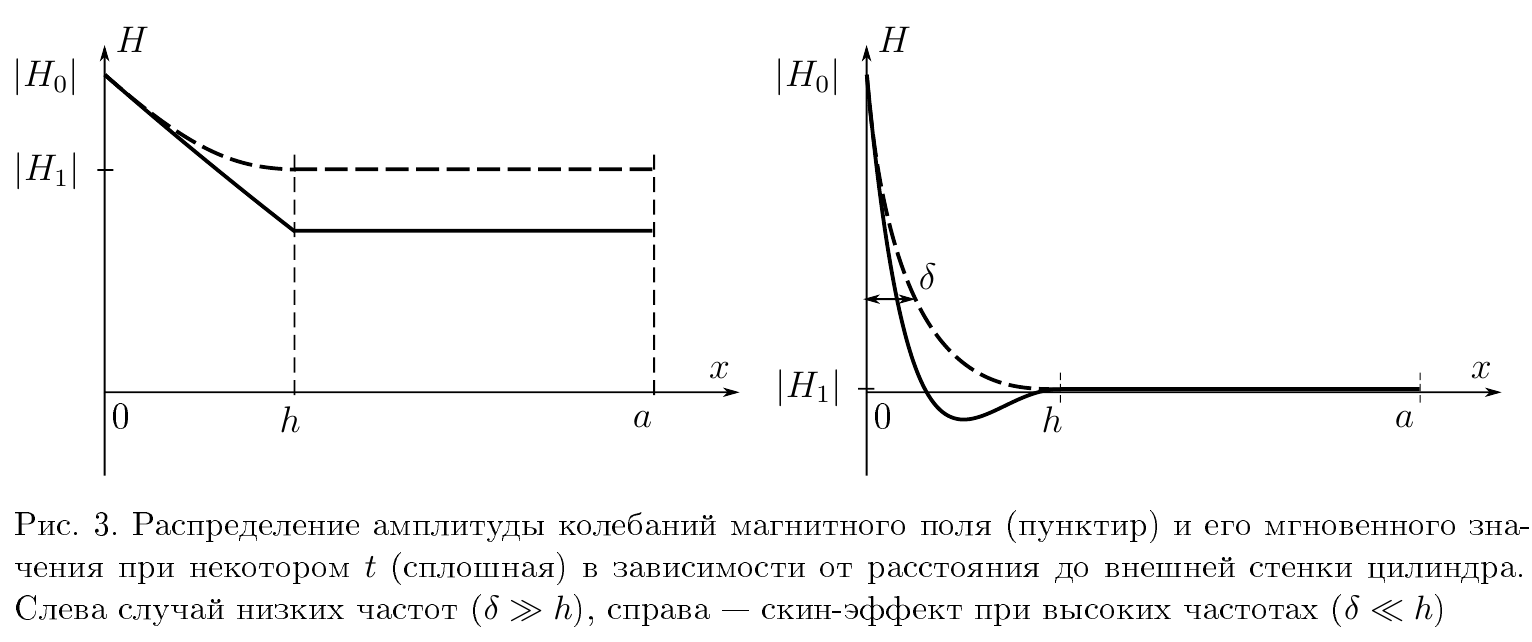
\includegraphics[width=0.8\linewidth]{../img/fig3.png}}
\end{figure}

 
 
